\definecolor{gold}{rgb}{0.77,0.69,0.37}
\newlength{\hptitlewidth}
\newlength{\rationalh}
\newcommand{\hptitle}[2][\stockwidth]{%
\setlength{\hptitlewidth}{#1}%
\centering\color{white}%
\vskip 3cm\resizebox{.95\hptitlewidth}{!}{\textls[100]{HARRY POTTER AND THE}}%
\vskip 2mm%
\color{gold}%
\settoheight{\rationalh}{\resizebox{.95\hptitlewidth}{!}{\textls[20]{RATIONALITY}}}
\resizebox{!}{0.9\rationalh}{\textls[50]{METHODS}}%
\hfil\resizebox{!}{0.3\rationalh}{\textls[50]{Of}}%
\vskip 2mm%
\resizebox{.95\hptitlewidth}{!}{\textls[20]{RATIONALITY}}%
\vskip 8mm%
\color{white}%
\resizebox{.5\hptitlewidth}{!}{\textls[50]{\scshape{}Fanfiction von Eliezer Yudkowsky}}%
\vskip 4mm%
\resizebox{.35\hptitlewidth}{!}{\textls[50]{\scshape{}Deutsche Übersetzung}}%
\vfill%
\textls[50]{\scshape #2}%
\color{black}%
\vskip 1cm\ %
}
\providecommand{\fullvolumetitle}[1]{Buch #1: \volumetitle}

\ifcover%
\definecolor{backgroundcover}{HTML}{272c36}
\newpagecolor{backgroundcover}\afterpage{\restorepagecolor}
\newcommand\BackgroundPic{
\put(0,0){%
\parbox[b][\paperheight]{\paperwidth}{%
\vfill%
\centering%
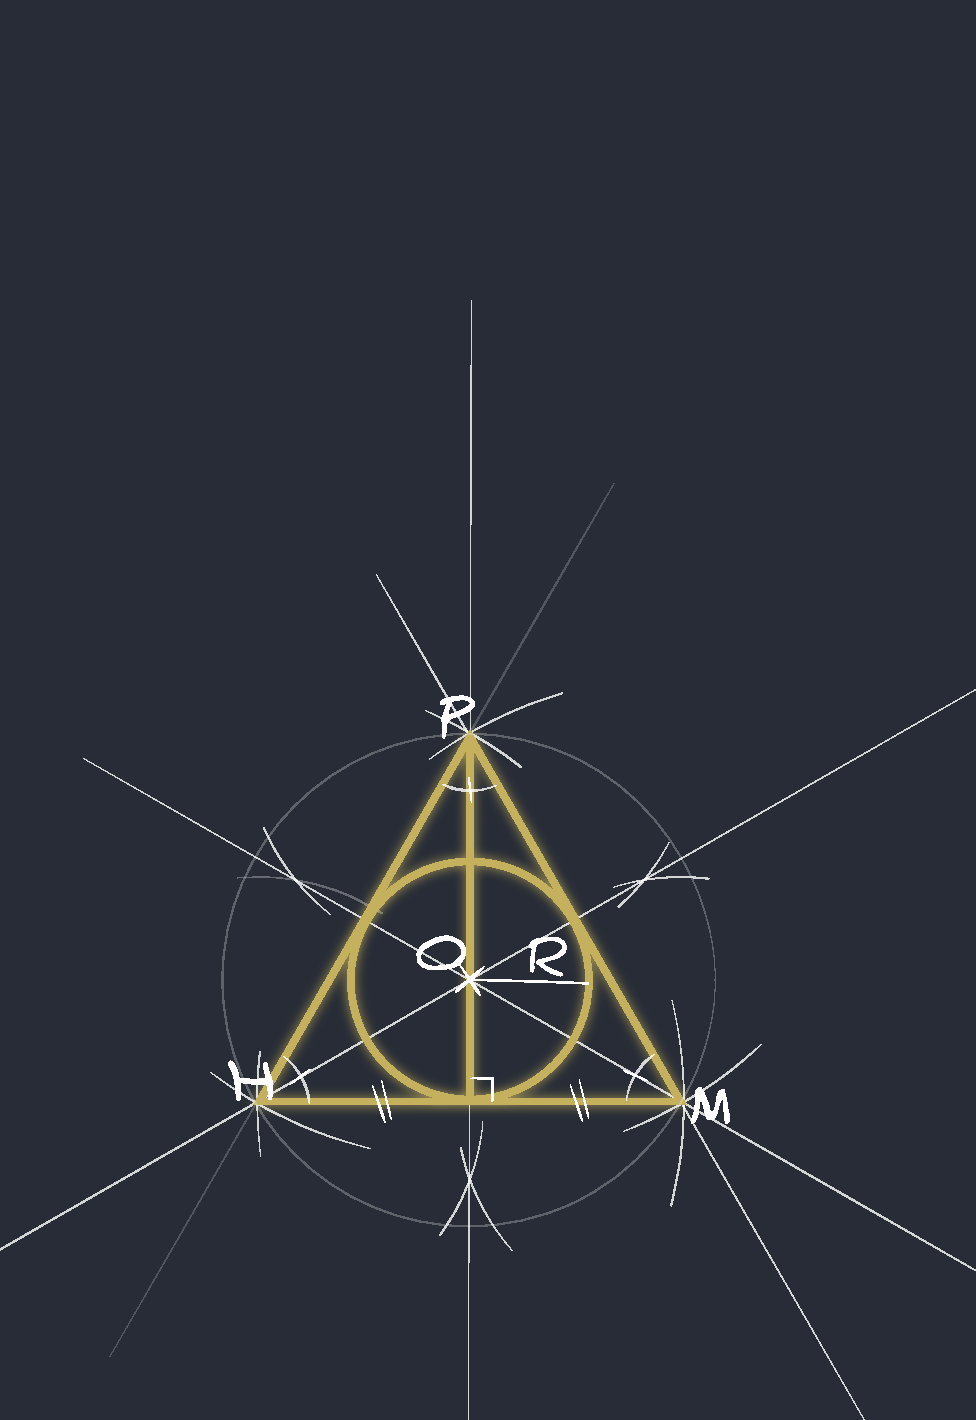
\includegraphics[width=\paperwidth,height=\paperheight,keepaspectratio]{images/cover1.pdf}%
\vfill%
}}}\AddToShipoutPicture*{\BackgroundPic}%
\AddToShipoutPicture*{\put(0,0){%
\parbox[b][\paperheight]{\paperwidth}{%
\hptitle{\fullvolumetitle{\volumenumber}}%
}}}%
\ %
\cleartorecto
\fi

\begin{center}
\thispagestyle{empty}
\vspace*{0.5cm}
\makebox[0pt][c]{%
  \raisebox{-\totalheight}[0pt][0pt]{%
    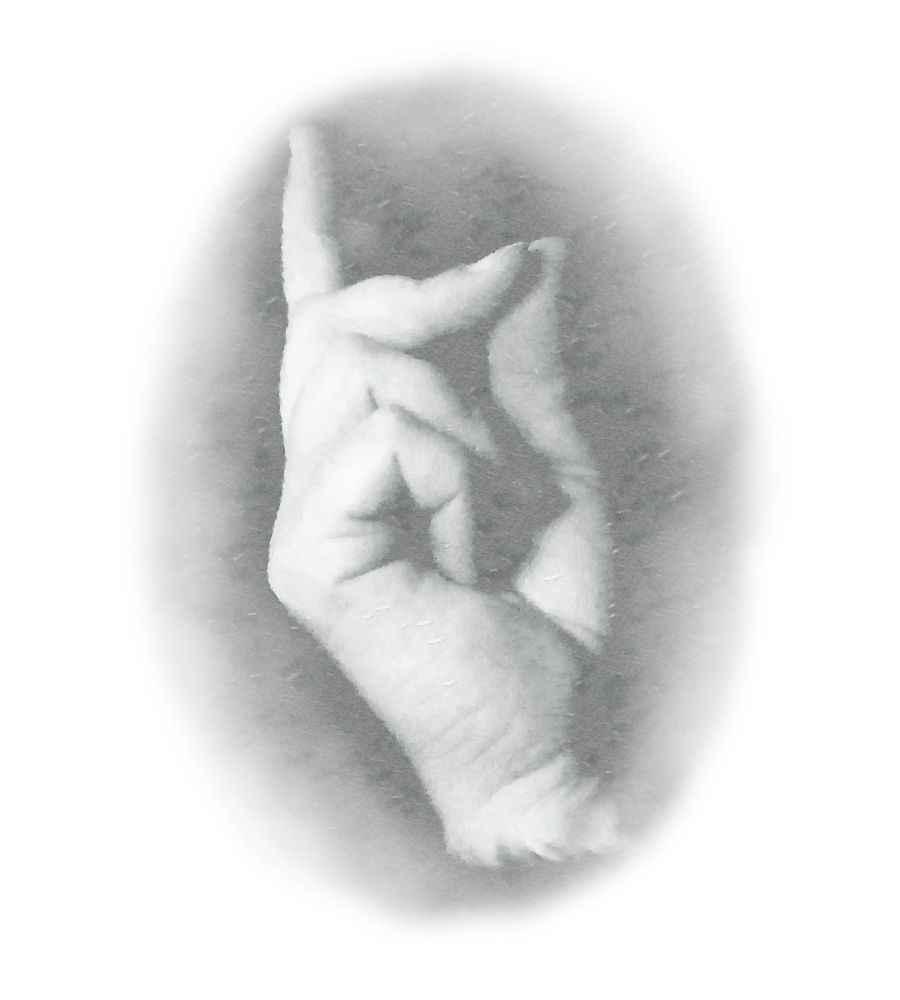
\includegraphics[scale=0.75]{images/cover0.jpg}}}%

\vspace*{-1.5cm}
{\hpfont
\Huge\MakeUppercase{Harry Potter}\vspace*{0.5cm}

\Large\MakeUppercase{and the Methods of Rationality} %
\vspace*{1\baselineskip}
% 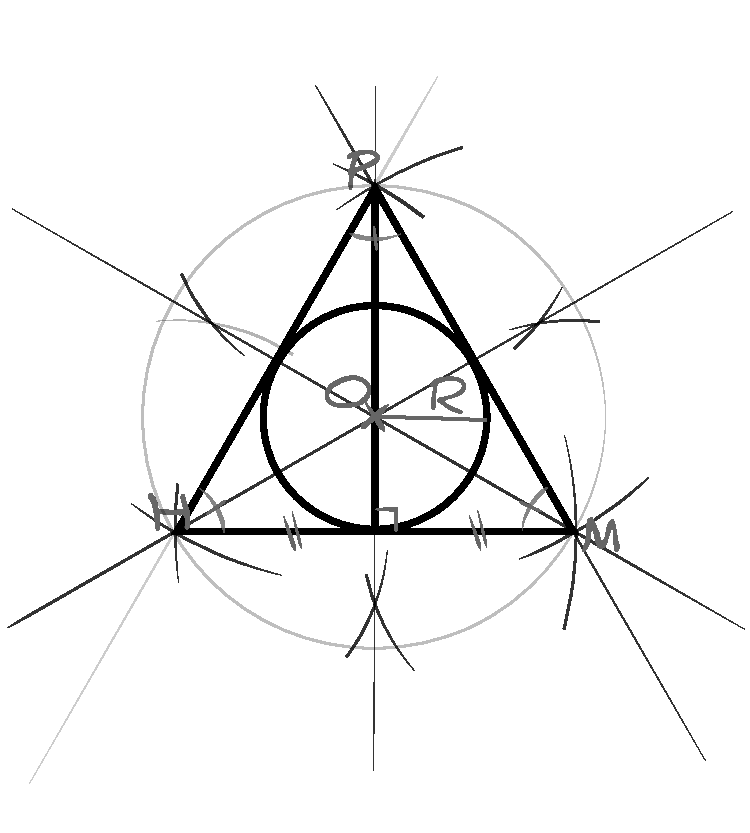
\includegraphics[scale=0.5]{images/cover2.pdf}




\vspace*{7.0cm}

% \vspace*{1\baselineskip}
\Large Fanfiction von \vspace*{.10cm}

\huge \MakeUppercase{Eliezer Yudkowsky}%

\small

\vspace*{1\baselineskip}
Basierend auf der Harry Potter Reihe von J.~K.~Rowling\\
}
\vfill
{
\vspace*{1\baselineskip}
Author's disclaimer:\\J.~K.~Rowling owns Harry Potter, and no one owns the methods of rationality.
% Disclaimer: ~K.~Rowling besitzt alle Rechte an Harry Potter, aber niemandem gehören die Methods of Rationality.
\\\vspace*{1\baselineskip}
Die englische Originalfassung gibt es unter {\small\href{http://hpmor.com}{http://hpmor.com}}\\
und als überarbeites PDF und eBook unter\\
{\small\href{https://github.com/rrthomas/hpmor/}{github.com/rrthomas/hpmor/}}\\
%\\\vspace*{1\baselineskip}\fullvolumetitle{\volumenumber}
}
\end{center}


\newpage
\begin{center}
\noindent
\vfill
Dies ist ein \href{https://github.com/entorb/hpmor-de/}{OpenSource Projekt}\\
gestartet von \href{https://entorb.net}{Torben Menke}\\
{\small\href{https://github.com/entorb/hpmor-de/}{github.com/entorb/hpmor-de/}}\\

\vspace*{1\baselineskip}
Verbesserungsvorschläge und Mitarbeit sind herzlich willkommen\\
unter {\small\href{https://github.com/entorb/hpmor-de/wiki/Mitmachen}{github.com/entorb/hpmor-de/wiki/Mitmachen}}\\

\vspace*{1\baselineskip}
Großer Dank gebührt den initialen Übersetzern\\
Jost (Kapitel 1-21) {\small\href{https://www.fanfiktion.de/s/4cb8beb50000203e067007d0/}{fanfiktion.de/s/4cb8beb50000203e067007d0/}}\\
Patneu (Kapitel 22-38) {\small\href{https://www.fanfiktion.de/s/55610c610004dede273a3811/}{fanfiktion.de/s/55610c610004dede273a3811/}}\\
DieFuechsin (Kapitel 39-78) {\small\href{https://www.fanfiktion.de/s/5c793dfe000a402030774dc7/}{fanfiktion.de/s/5c793dfe000a402030774dc7/}}\\
Schneefl0cke (Kapitel 79-122) {\small\href{https://www.fanfiktion.de/s/60044849000ccc541aef297e/}{fanfiktion.de/s/60044849000ccc541aef297e/}}\\

\vspace*{1\baselineskip}
Sowie den Kollegen der anderssprachigen Ausgaben für den tollen\\
Austausch von Ideen, Quellcode, Layout und Schriften\\
{\small\href{https://github.com/rrthomas/hpmor/}{github.com/rrthomas/hpmor/}} (EN)\\
{\small\href{https://github.com/yeKcim/hpmor/}{github.com/yeKcim/hpmor/}} (FR)\\

\vspace*{1\baselineskip}
Version vom \today{}

\vspace*{1\baselineskip}
Das neuste PDF und eBook gibt es unter\\
{\small\href{https://github.com/entorb/hpmor-de/releases/tag/WorkInProgress}{github.com/entorb/hpmor-de/releases/tag/WorkInProgress}}\\
\end{center}
